% !TeX spellcheck = it_IT
\documentclass[10pt,a4paper]{article}

\usepackage[utf8]{inputenc}
\usepackage[T1]{fontenc}	
\usepackage[italian]{babel}
\usepackage{amsmath}
\usepackage{amsfonts}
\usepackage{amssymb}
\usepackage{graphicx}

\usepackage[left=2cm,right=2cm,top=2cm,bottom=2cm]{geometry}
\geometry{a4paper}

\usepackage{booktabs} % for much better looking tables
\usepackage{verbatim}
\usepackage{subfig} % make it possible to include more than one captioned figure/table in a single 

\usepackage{fancyhdr} % This should be set AFTER setting up the page geometry
\pagestyle{fancy} % options: empty , plain , fancy
\renewcommand{\headrulewidth}{0pt} % customise the layout...
\lhead{}\chead{}\rhead{}
\lfoot{}\cfoot{\thepage}\rfoot{}

%%% SECTION TITLE APPEARANCE
\usepackage{sectsty}
%\allsectionsfont{\sffamily\mdseries\upshape} % (See the fntguide.pdf for font help)
% (This matches ConTeXt defaults)

% pacchetti che mi fanno schifo ma uso lo stesso (Bob è scemo, ma anche Ale...)
\usepackage[cdot, thickqspace, squaren]{SIunits}
% macro che mi piacciono
\def\code#1{\texttt{#1}}


\title{Esercitazione 5: Transistor JFET}

\author{Gruppo BE \\ Alessandro Candido, Roberto Ribatti}
\date{\today}
\begin{document}
\maketitle

\section{Scopo e strumentazione}
Studiare le caratteristiche e realizzare un amplificatore con il JFET a canale N 2N3819.
La strumentazione usata è quella presente sul banco di lavoro, più il suddetto transistor.

\section{Studio del funzionamento del JFET}

\subsection{Dimensionamento}
Si è montato il circuito in \figurename{\ref{fig:circuito1}}.

\begin{figure}[h!]
	\centering
	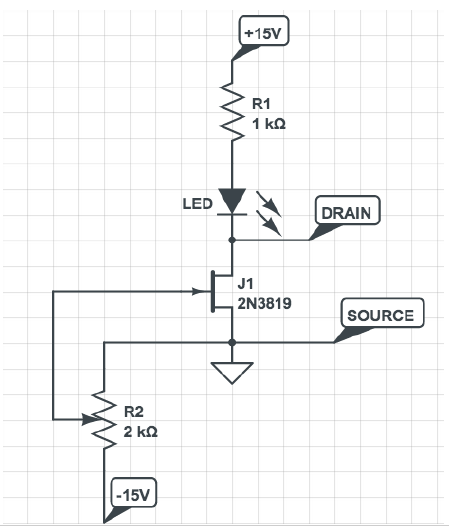
\includegraphics[width=0.4\textwidth]{../grafici/Circuito1.png}
	\caption{Circuito per lo studio del funzionamento del JFET}
	\label{fig:circuito1}
\end{figure}

I valori dei componenti usati sono stati misurati con il multimetro digitale.

\begin{table}[h!]
	\centering
	\begin{tabular}{ccc}
		$V_{15} = \unit{15.0 \pm 0.2}{\volt}$  & $V_{-15} = \unit{-15.0 \pm 0.2}{\volt}$ & $R_1 = \unit{985 \pm 9}{\ohm}$
	\end{tabular}
\end{table}

\paragraph{LED} Il LED si accende e si spegne alla tensione $V_{GS} \sim \unit{1.9}{\volt}$. Infatti al di sopra di una certa tensione gate-source ($V_{GS}$) il canale è da considerarsi chiuso (pinch-off) e il transistor va in interdizione. Al di sotto della tensione di pinch-off la corrente inizia a scorrere nel canale, portando in conduzione anche il LED.

\subsection{Tensione di pinch-off $V_P$ e massima corrente di drain $I_{DSS}$}
I dati relativi alla curva $I_D - V_{GS}$ sono riportati in appendice in \tablename{\ref{njfet}}, il grafico relativo è invece riportato di seguito in \figurename{\ref{fig:njfet}}.

\begin{figure}[h!]
	\centering
	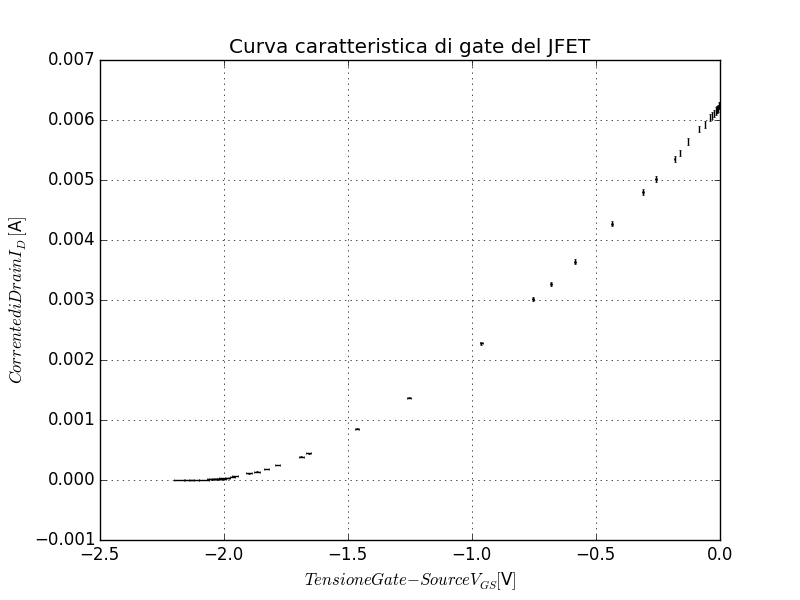
\includegraphics[width=0.8\textwidth]{../grafici/fast_plot_caratterizzazioneJFET.pdf}
	\caption{Curva caratteristica di gate del JFET}
	\label{fig:njfet}
\end{figure}

Si è trovato per la tensione di pinch-off il valore di $V_P = \unit{-2.198 \pm 0.025}{\volt} $, mentre per la massima corrente di drain $I_{DSS} = {6.24 \pm 0.06 }{\milli\ampere} $.

\subsection{Nota sulla stima di $V_P$}
Per misurare il valore della tensione di pinch-off si è applicata la definizione, cioé la tensione a cui il canale si chiude completamente. Si è interpretata in questo caso come il valore della tensione a cui la corrente di drain si annulla (infatti a canale chiuso rimane solo il semiconduttore drogato, che ha una conducibilità nettamente inferiore al conduttore ohmico in cui avviene il trasporto di carica a canale aperto).

Si è notato però che, oltre all'incertezza di lettura del multimetro su tale tensione, era da propagare anche l'incertezza con cui era noto che il valore della corrente fosse nullo.

\begin{figure}[h!]
	\centering
	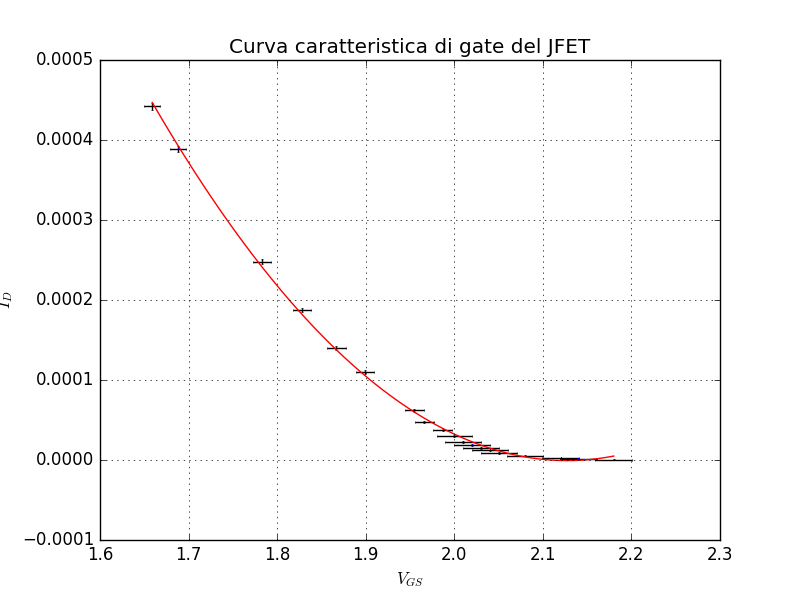
\includegraphics[width=0.6\textwidth]{../grafici/fit_carattx2.pdf}
	\caption{Grafico del fit usato per ricavare $V_P$}
	\label{fig:vpfit}
\end{figure}

Per propagare tale valore si è cercato di approssimare la curva che descrivevano i dati con la sua espansione di Taylor, dato che non era nota la curva teorica (la conosceremmo se sapessimo di essere in saturazione).
Dall'osservazione del grafico si deduce però che la curva ha una concavità abbastanza accentuata, per cui la tangente alla curva è sempre più orizzontale. A questo punto si ha che il termine dominante nell'espansione potrebbe non essere l'ordine lineare, come confermato in prima battuta dall'osservazione dei punti, si è dunque approssimata la curva con un espansione al second'ordine, imponendo che raggiungesse il suo minimo per una corrente di drain nulla.

Infine il valore di $V_P$ è stato ottenuto dal fit dei punti più prossimi (5 in particolare) al minimo con una funzione della forma $I_D(V_{GS}) = a(V_{GS} - V_P)^2$, ottenendo per $V_P$ il valore riportato e un $\chi^2 / ndof = 2.16 / 3$, il grafico è riportato in figura \figurename{\ref{fig:vpfit}}.

Va notato che, ipotizzando di essere veramente in saturazione, la formula utilizzata per il fit è esattamente la curva attesa, con $a = k_P$.

%aggiungere grafico fit

\section{Montaggio amplificatore}

\subsection{Dimensionamento}

I valori dei componenti usati nel circuito in \figurename{\ref{fig:amplificatore}} sono:

\begin{table}[h!]
\centering
\begin{tabular}{cccc}
$R_1 = \unit{985 \pm 9}{\ohm}$ & $R_3 = \unit{4.65 \pm 0.07}{\mega\ohm}$ & $R_{trim} = \unit{244 \pm 3}{\ohm}$ & $ C_1 = \unit{101 \pm 5}{\nano\farad}$
\end{tabular}
\end{table}

Si è indicato con $R_{trim}$ la resistenza del potenziometro al punto di lavoro fissato (si veda paragrafo seguente).

\begin{figure}[h!]
	\centering
	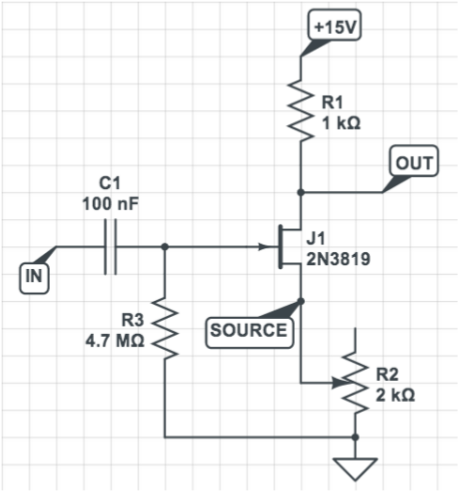
\includegraphics[width=0.4\textwidth]{../grafici/amplificatore.png}
	\caption{Schema del circuito dell'amplificatore a JFET (common source o source follower)}
	\label{fig:amplificatore}
\end{figure}

\paragraph{Punto di lavoro} Si è montato l'amplificatore, rappresentato in \figurename{\ref{fig:amplificatore}}, imponendo il punto di lavoro in modo tale che la corrente di drain $I_D$ fosse $\sim I_{DSS}/2$. Il valore misurato è $I_D = \unit{3.05 \pm 0.03}{\milli\ampere}$.

%I valori misurati per tensione drain-source e corrente di drain sono riportati di seguito.
%\begin{table}[h!]
%\centering
%\begin{tabular}{cc}
%$V_{DS} = \unit{650 \pm 4}{\volt}$ & $I_{DS} = \unit{3.05 \pm 0.03}{\milli\ampere}$
%\end{tabular}
%\end{table}

Si è misurato inoltre $V_{GS} = \unit{650 \pm 4}{\milli\volt}$ e si è calcolato il valore atteso per la corrente di drain $I_D$ secondo la formula:
\begin{equation*}
I_D = \frac{I_{DSS}}{V_P^2}(V_{GS} - V_P)^2
\end{equation*}

Ottenendo quindi $I_D^{exp} = \unit{3.10 \pm 0.04}{\milli\ampere}$ che è in accordo con quello misurato. Si ottiene inoltre per la transconduttanza il valore di $g_m = \unit{3.98 \pm 0.06}{\milli\siemens}$.
%i valori sono ottenuti con Vp e Idss presi a spanne con errori dal multimetro, poi lo aggiorno, comunque sono già compatibili

\section{Misure a frequenza fissa}

Si è misurato il guadagno in risposta a segnali sinusoidali di frequenza fissa pari a $\unit{1.011 \pm 0.010}{k\hertz}$ nella configurazione di common source e source follower.

\paragraph{Fase relativa tra ingresso e uscita} Si è osservato che il segnale in uscita risultava in opposizione di fase rispetto al segnale in ingresso nel caso della configurazione common source e in fase nel caso della configurazione source follower, come atteso. Si riporta in \figurename{\ref{fig:controfase}} e \figurename{\ref{infase}} le relative schermate dell'oscilloscopio.

\begin{figure}[h!]
	\centering
	\begin{minipage}[h!]{0.45\textwidth}
		\centering
		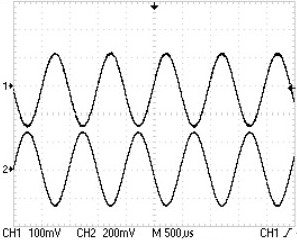
\includegraphics[width=\textwidth]{../oscilloscopio/inversione_fase.jpg}
		\caption{common source}
			\label{fig:controfase}
	\end{minipage}
	\begin{minipage}[h!]{0.45\textwidth}
		\centering
		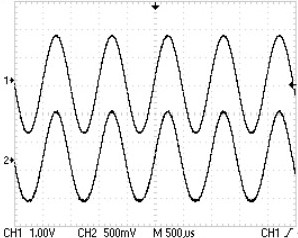
\includegraphics[width=\textwidth]{../oscilloscopio/fase.jpg}
		\caption{source follower}
			\label{infase}
	\end{minipage}
\end{figure}

\paragraph{Guadagno e linearità del circuito} Si è fittato il guadagno in tensione del circuito $|A_V|$ ottenendo i seguenti risultati:

\begin{table}[h!]
	\centering
	\begin{tabular}{c|ccc}
		common source & $|A_v| = 1.996 \pm 0.019$ & intercetta: $\unit{0.005 \pm 0.008}{\volt}$ & $\chi^2 / ndof = 25.5 / 22$\\
		source follower &	$|A_v| = 0.470 \pm 0.005$ & intercetta: $\unit{0.0025 \pm 0.0012}{\volt}$ & $\chi^2 / ndof = 21.3 / 23$
	\end{tabular}
\end{table}

Il valore atteso dalla teoria è di
\begin{table}[h!]
	\centering
	\begin{tabular}{c|c}
		common source & $|A_v|^{exp} =g_mR_1/(1+g_mR_{trim}) = 1.989 \pm 0.027$ \\
		source follower &	$|A_v|^{exp} =g_mR_1/(1+g_mR_{trim}) = 0.493 \pm 0.005$
	\end{tabular}
\end{table}

Il primo è in accordo con il valore misurato, mentre non lo è il secondo. Sospettiamo che possa essere imputato a piccole variazioni del valore della resistenza del trimmer che è stata misurata nel corso della presa dati.
I grafici dei fit sono riportati di seguito, mentre i dati raccolti sono in appendice in \tablename{\ref{tab:commonsource}} e \tablename{\ref{tab:sourcefollower}}.

\begin{figure}[h!]
	\centering
	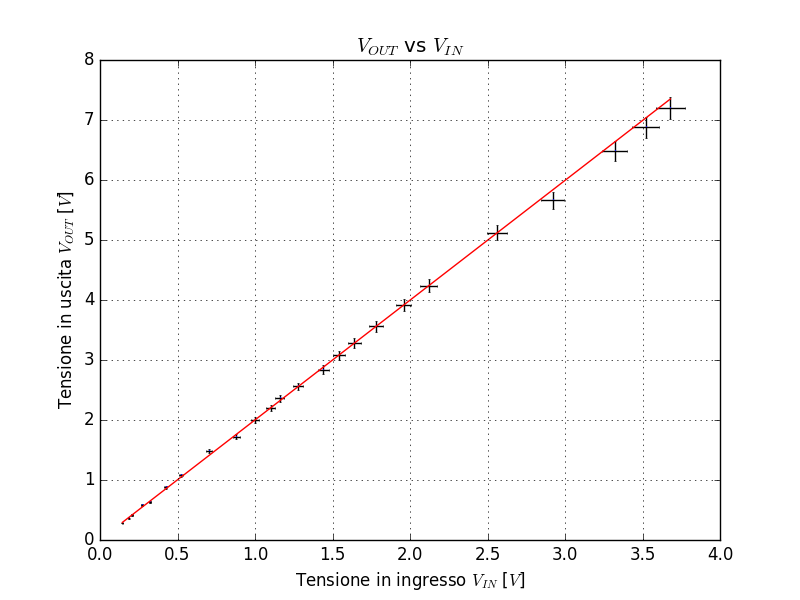
\includegraphics[width=0.75\textwidth]{../grafici/fit_guadagnovstensione.pdf}
	\caption{Grafico del fit del guadagno del circuito common source}
\end{figure}
\pagebreak
\begin{figure}[h!]
	\centering
	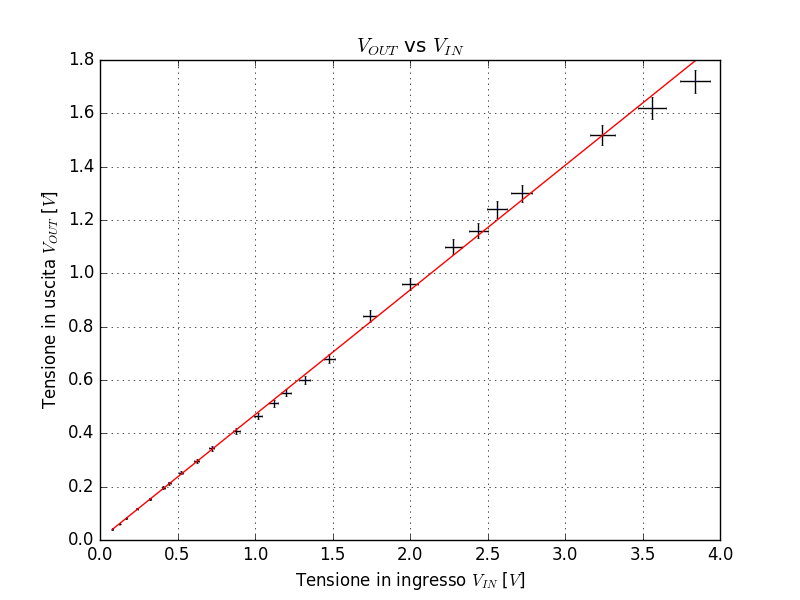
\includegraphics[width=0.75\textwidth]{../grafici/fit_guadagnovstensione2.pdf}
	\caption{Grafico del fit del guadagno del circuito source follower}
\end{figure}
 Si può affermare che la linearità è preservata per le tensioni d'ingresso che non portano il transistor in clipping.
  
 \paragraph{Clipping}
Il segnale in uscita risulta sinusoidale fino ad ampiezze di $\sim \unit{4.4}{\volt}$ in ingresso per entrambe le configurazioni.
Per intensità maggiori si osserva che l'uscita è tagliata dall'alto nel common source e dal basso nel source follower. Questo taglio del segnale (riportato in \figurename{\ref{fig:clippingalto}} e \figurename{\ref{fig:clippingbasso}}) corrisponde ad un regime di funzionamento del transistor diverso da quello attivo (interdizione), in cui sarebbe preservata la linearità.

\begin{figure}[h!]
	\centering
	\begin{minipage}{0.49\textwidth}
		\centering
		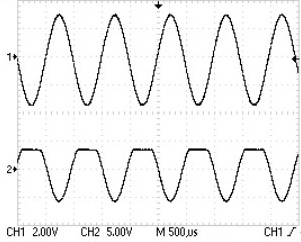
\includegraphics[width=\textwidth]{../oscilloscopio/clipalto.jpg}
		\caption{Clipping common source}                                                                          
			\label{fig:clippingalto}
	\end{minipage}
	\begin{minipage}{0.49\textwidth}
		\centering
		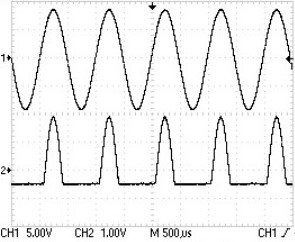
\includegraphics[width=\textwidth]{../oscilloscopio/clipbasso.jpg}
		\caption{Clipping source follower}	
			\label{fig:clippingbasso}	
	\end{minipage}
\end{figure}

\section{Impedenza d'ingresso}                                                                                                                                 
Si è cercato di misurare l'impedenza di ingresso del circuito per segnali a frequenza
$f_1 = \unit{1.011 \pm 0.010}{k\hertz}$ e $f_2= \unit{10.04 \pm 0.10}{k\hertz}$.

A questo scopo si è misurata la caduta di potenziale su una resistenza $R_S = \unit{677 \pm 6}{\kilo\ohm}$ (nel caso dei segnali a $\unit{1}{k\hertz}$) e $R_S' = \unit{178.1 \pm 2.7}{\kilo\ohm}$ (per i segnali a $\unit{10}{k\hertz}$) in serie al circuito, misurando il potenziale riferito a terra prima e dopo la resistenza.

I due potenziali sono:
\begin{table}[h!]
	\centering
	\begin{tabular}{c|cc}
		$\unit{1}{k\hertz}$ & $V_1 = \unit{2.80 \pm 0.10}{\volt}$  & $V_2 = \unit{1.42 \pm 0.05}{\volt}$\\
		$\unit{10}{k\hertz}$ & $V'_1 = \unit{2.84 \pm 0.10}{\volt}$  & $V'_2 = \unit{1.30 \pm 0.05}{\volt}$
	\end{tabular}
\end{table}

Per ottenere l'impedenza di ingresso bisognerà tenere conto che $V_2$ è la tensione sul parallelo tra questa e l'impedenza di ingresso dell'oscilloscopio che dalle esperienze precedenti è nota essere pari a $R_O=\unit{1.00 \pm 0.02}{\mega\ohm}$\footnote{Si potrebbe fare a meno di conoscere l'impedenza di ingresso se si fosse misurata la tensione all'output, questo perchè }. Per le impedenze di ingresso si ottiene quindi:
\begin{table}[h!]
	\centering
	\begin{tabular}{cc}
	$R_{IN}^{1k} = \unit{2.3 \pm 0.8}{\mega\ohm}$ & $R_{IN}^{10k} = \unit{177 \pm 19}{k\ohm}$
	\end{tabular}
\end{table}

Nel caso teorico ideale l'impedenza di ingresso del transistor è infinita e l'impedenza del circuito dovrebbe essere pari a $R_G$ cioè $\sim\unit{4.7}{\mega\ohm}$, è evidente però che in questo caso questa approssimazione non è applicabile e che l'impedenza di ingresso del transistor è complessa, dovuta evidentemente alla capacità delle giunzioni. Nell'ipotesi che l'impedenza del transistor sia totalmente dovuta ad una capacità e che la resistenza di source $R_{trim}$ in serie sia trascurabile, si ottiene una stima della capacità di:
\begin{table}[h!]
	\centering
	\begin{tabular}{cc}
		$C^{1k} = \unit{6.0 \pm 2.7}{\pico\farad}$ & $C^{10k} = \unit{9.0 \pm 1.0}{\pico\farad}$
	\end{tabular}
\end{table}

Questi valori sono compatibili fra loro entro $\sim 1\sigma$ e sono comparabili alla capacità totale del transistor dichiarata sul datasheet (valore tipico di $\sim \unit{3}{\pico\farad}$ e massimo di $\sim \unit{12}{\pico\farad}$).

\section{Aumento del guadagno}

Si è proceduto alla ricerca della massima amplificazione modificando il punto di lavoro attraverso la rotazione del potenziometro.
    
Teoricamente ci aspettiamo che il massimo sia raggiunto per il valore minimo della resistenza del potenziometro.
Il guadagno è infatti dato da $|A_v| =g_mR_D/(1+g_mR_S)$: per $R_S\sim\unit{0}{\ohm}$ ho il valore massimo di corrente di drain e conseguentemente il massimo valore di $g_m = 2 \sqrt{(I_{DSS}*I_D)}/|V_P|$, inoltre ho il minimo del denominatore per cui il guadagno diventa:
\begin{equation*}
|A_v|^{exp} = \frac{2 I_{DSS}*R_D}{|V_P|} = 5.59 \pm 0.08 
\end{equation*}
I risultati delle misure sono stati:
\begin{table}[h!]
	\centering
	\begin{tabular}{ccc}
		$V_{IN}=\unit{740 \pm 20}{m\volt}$ & $V_{OUT} = \unit{3.60 \pm 0.09}{\volt}$ & $|A_v| = 4.86 \pm 0.18$\\
	\end{tabular}
\end{table}

I valori misurati si discostano da quelli attesi perché, per $R_S \sim 0$, il segnale in uscita andava in clipping, e dunque riduceva necessariamente il valore del guadagno rispetto a quello atteso, in questo regime infatti la formula usata per la transconduttanza non è più valida.

\pagebreak
\section{Appendice: Dati}
Si riportano qui le tabelle di dati usati per i fit e i grafici.

\centering
\begin{figure}[h!]
	\begin{minipage}[t]{0.33\textwidth}
		\centering
		\resizebox{1\textwidth}{!}{
		\input{../tabelle/tab_caratterizzazioneJFET1.txt}}
		\captionof{table}{Curva $I_D - V_{GS}$}
		\label{njfet}
	\end{minipage}
	\begin{minipage}[t]{0.33\textwidth}
		\resizebox{1\textwidth}{!}{
		\input{../tabelle/tab_linearity2.txt}}
		\captionof{table}{Gain common source}
		\label{tab:commonsource}
	\end{minipage}
	\begin{minipage}[t]{0.32\textwidth}
		\centering
		\resizebox{1\textwidth}{!}{
		\input{../tabelle/tab_linearity.txt}}
		\captionof{table}{Gain source follower}
		\label{tab:sourcefollower}
	\end{minipage}
\end{figure}

\end{document}
